\documentclass{article}
\usepackage[a4paper, margin=0.5in]{geometry}
\usepackage{tikz}
\usetikzlibrary{shapes.geometric, arrows.meta, positioning, fit, calc, backgrounds, shadows.blur}

\begin{document}

\begin{figure}[ht]
\centering
\resizebox{0.95\textwidth}{!}{%
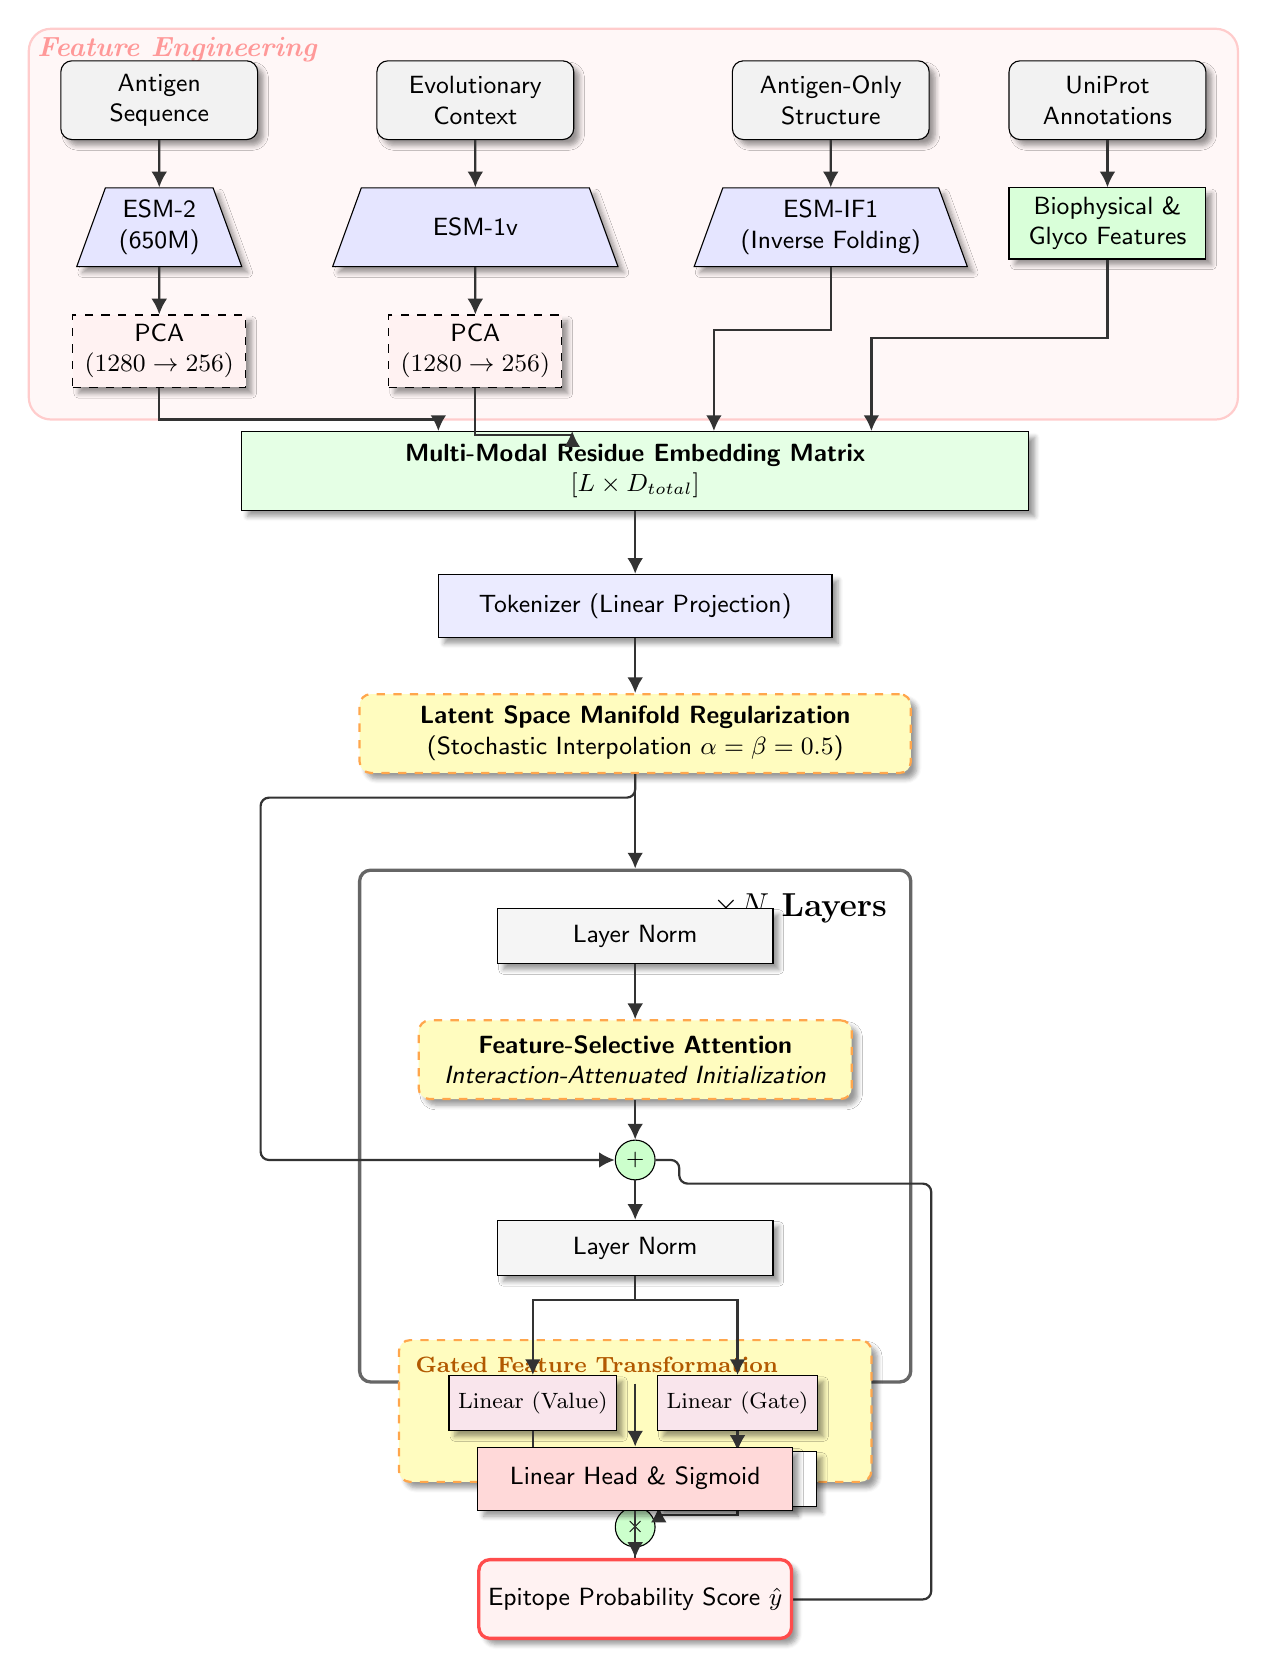
\begin{tikzpicture}[
    node distance=0.8cm and 0.8cm,
    font=\sffamily\small,
    >={Latex[width=2mm,length=2mm]},
    % Styles
    base/.style = {draw, align=center, blur shadow={shadow blur steps=5}},
    input/.style = {base, rectangle, rounded corners, fill=gray!10, minimum height=1cm, minimum width=2.5cm},
    model/.style = {base, trapezium, trapezium angle=70, fill=blue!10, minimum height=1cm, minimum width=2cm},
    process/.style = {base, rectangle, fill=orange!10, minimum height=0.8cm, minimum width=2.5cm},
    pca/.style = {base, rectangle, fill=pink!20, dashed, minimum height=0.7cm, minimum width=2.2cm},
    tensor/.style = {base, rectangle, fill=green!10, minimum height=1cm, minimum width=10cm},
    block/.style = {draw, rectangle, rounded corners, fill=white, draw=black!60, very thick, minimum width=7cm, minimum height=6.5cm},
    op/.style = {circle, draw, fill=green!20, inner sep=2pt, font=\footnotesize\bfseries},
    novelty/.style = {base, rectangle, rounded corners, fill=yellow!25, draw=orange!70, dashed, thick},
    normbox/.style = {base, rectangle, fill=gray!8, minimum height=0.7cm, minimum width=3.5cm},
    glubox/.style = {base, rectangle, fill=orange!8, minimum height=0.7cm, minimum width=2cm, font=\footnotesize},
    line/.style = {draw, ->, thick, black!80}
]

% ---------------------------------------------------------
% 1. Input and Feature Extraction Layer
% ---------------------------------------------------------

% Sequence Branch (Left)
\node[input] (seq) {Antigen\\Sequence};
\node[input, right=1.5cm of seq] (seq2) {Evolutionary\\Context};

% Models below inputs
\node[model, below=0.6cm of seq] (esm2) {ESM-2\\(650M)};
\node[model, below=0.6cm of seq2] (esm1v) {ESM-1v};

% Structure Branch (Right)
\node[input, right=2cm of seq2] (struct) {Antigen-Only\\Structure};
\node[input, right=1cm of struct] (annotations) {UniProt\\Annotations};

% Models below structure inputs
\node[model, below=0.6cm of struct] (esmif) {ESM-IF1\\(Inverse Folding)};
\node[process, below=0.6cm of annotations, fill=green!15] (features) {Biophysical \&\\Glyco Features};

% Arrows inputs to models
\draw[line] (seq) -- (esm2);
\draw[line] (seq2) -- (esm1v);
\draw[line] (struct) -- (esmif);
\draw[line] (annotations) -- (features);

% ---------------------------------------------------------
% 2. Dimensionality Reduction (PCA)
% ---------------------------------------------------------

\node[pca, below=0.6cm of esm2] (pca2) {PCA\\$(1280 \to 256)$};
\node[pca, below=0.6cm of esm1v] (pca1v) {PCA\\$(1280 \to 256)$};

\draw[line] (esm2) -- (pca2);
\draw[line] (esm1v) -- (pca1v);

% ---------------------------------------------------------
% 3. Concatenation
% ---------------------------------------------------------

% Calculate center position for concatenation tensor
\coordinate (mid_point) at ($(pca1v.east)!0.5!(esmif.west)$);
\node[tensor, below=1.8cm of mid_point] (concat) {\textbf{Multi-Modal Residue Embedding Matrix}\\$[L \times D_{total}]$};

% Connecting lines to Concat - using proper bending
\draw[line] (pca2.south) -- ++(0,-0.4) -| ([xshift=-2.5cm]concat.north);
\draw[line] (pca1v.south) -- ++(0,-0.6) -| ([xshift=-0.8cm]concat.north);
\draw[line] (esmif.south) -- ++(0,-0.8) -| ([xshift=1cm]concat.north);
\draw[line] (features.south) -- ++(0,-1.0) -| ([xshift=3cm]concat.north);

% ---------------------------------------------------------
% 4. Core Network Architecture
% ---------------------------------------------------------

% Tokenizer
\node[process, below=0.8cm of concat, fill=blue!8, minimum width=5cm] (token) {Tokenizer (Linear Projection)};
\draw[line] (concat) -- (token);

% Mixup (Novelty)
\node[novelty, below=0.7cm of token, minimum width=7cm, minimum height=1cm] (mixup) {\textbf{Latent Space Manifold Regularization}\\(Stochastic Interpolation $\alpha=\beta=0.5$)};
\draw[line] (token) -- (mixup);

% Transformer Block Container
\node[block, below=1.2cm of mixup] (transformer) {};
\node[anchor=north east, font=\bfseries\large] at ([xshift=-0.2cm, yshift=-0.2cm]transformer.north east) {$\times N$ Layers};

% -- Inside Transformer Block --

% Layer Norm 1
\node[normbox, below=0.5cm of transformer.north] (ln1) {Layer Norm};

% Attention (Novelty)
\node[novelty, below=0.7cm of ln1, minimum width=5.5cm, minimum height=1cm] (attn) {\textbf{Feature-Selective Attention}\\\textit{Interaction-Attenuated Initialization}};

% Residual Add 1
\node[op, below=0.5cm of attn] (add1) {$+$};

% Layer Norm 2
\node[normbox, below=0.5cm of add1] (ln2) {Layer Norm};

% GLU Container Box
\node[novelty, below=0.8cm of ln2, minimum width=6cm, minimum height=1.8cm] (glu_container) {};
\node[anchor=north west, font=\bfseries\footnotesize, text=orange!70!black] at ([xshift=0.1cm, yshift=-0.1cm]glu_container.north west) {Gated Feature Transformation};

% GLU Internals - positioned inside the container
\node[glubox, fill=purple!10] at ([xshift=-1.3cm, yshift=0.1cm]glu_container.center) (linear_v) {Linear (Value)};
\node[glubox, fill=purple!10] at ([xshift=1.3cm, yshift=0.1cm]glu_container.center) (linear_g) {Linear (Gate)};
\node[glubox, fill=white, below=0.25cm of linear_g] (act) {Sigmoid};

% Multiply operation
\node[op, below=0.3cm of glu_container] (mult) {$\times$};

% Residual Add 2
\node[op, below=0.4cm of mult] (add2) {$+$};

% -- Transformer Internal Connections --
\draw[line] (ln1) -- (attn);
\draw[line] (attn) -- (add1);
\draw[line] (add1) -- (ln2);

% Connections from LN2 to GLU internals
\draw[line] (ln2.south) -- ++(0,-0.3) -| (linear_v.north);
\draw[line] (ln2.south) -- ++(0,-0.3) -| (linear_g.north);
\draw[line] (linear_g) -- (act);

% GLU to multiply
\draw[line] (linear_v.south) -- ++(0,-0.55) -| ([xshift=-0.3cm]mult.north);
\draw[line] (act.south) -- ++(0,-0.1) -| ([xshift=0.3cm]mult.north);
\draw[line] (mult) -- (add2);

% Residual Connections (bypass arrows)
% Residual 1: from before LN1 to add1
\coordinate (res1_start) at ([xshift=-3cm]ln1.west);
\draw[line, rounded corners=3pt] (mixup.south) -- ++(0,-0.3) -| (res1_start) |- (add1.west);

% Residual 2: from add1 output to add2
\coordinate (res2_start) at ([xshift=-3cm]ln2.west);
\draw[line, rounded corners=3pt] (add1.east) -- ++(0.3,0) -- ++(0,-0.3) -- ++(3.2,0) |- (add2.east);

% Connection from mixup to transformer
\draw[line] (mixup) -- (transformer.north);
\draw[line, draw=none] (transformer.north) -- (ln1); % internal flow

% ---------------------------------------------------------
% 5. Output Head
% ---------------------------------------------------------

\node[process, below=0.8cm of transformer, fill=red!15, minimum width=4cm] (head) {Linear Head \& Sigmoid};
\node[input, below=0.6cm of head, draw=red!70, very thick, fill=red!5] (output) {Epitope Probability Score $\hat{y}$};

\draw[line] (transformer.south) -- (head);
\draw[line] (head) -- (output);

% ---------------------------------------------------------
% Background Box for Feature Engineering
% ---------------------------------------------------------

\begin{scope}[on background layer]
    \node[fit=(seq)(seq2)(struct)(annotations)(esm2)(esm1v)(esmif)(features)(pca2)(pca1v), 
          fill=red!3, rounded corners=8pt, draw=red!20, thick,
          inner sep=0.4cm,
          label={[anchor=north west, font=\bfseries\itshape, text=red!40]north west:Feature Engineering}] {};
\end{scope}

\end{tikzpicture}
}
\caption{Schematic overview of the Glyco-EpitopeTransformer architecture. Multi-modal inputs are processed via pre-trained ESM models and biophysical calculations. High-dimensional embeddings are reduced via PCA and concatenated. The core network utilizes Latent Space Manifold Regularization (Mixup) before passing through Transformer blocks modified with Feature-Selective Attention (using attenuated initialization) and Gated Linear Units (GLU) to handle complex, noisy biophysical data.}
\label{fig:network_architecture}
\end{figure}

\end{document}
